\documentclass[16 pt]{amsart}
\usepackage{amscd,amsmath,amsthm,amssymb}
\usepackage{enumerate,varioref}
\usepackage{epsfig}
\usepackage{graphicx}
\usepackage{mathtools}
\usepackage{tikz}
\usepackage{lscape}
\newtheorem{thm}{Theorem}
\newtheorem{cor}[thm]{Corollary}
\newtheorem{lem}[thm]{Lemma}
\newtheorem{prop}[thm]{Proposition}
\theoremstyle{definition}
\newtheorem{defn}[thm]{Definition}
\theoremstyle{remark}
\newtheorem{ex}[thm]{Example}
\newtheorem{rem}[thm]{Remark}
\begin{document}

%\begin{landscape}
\[
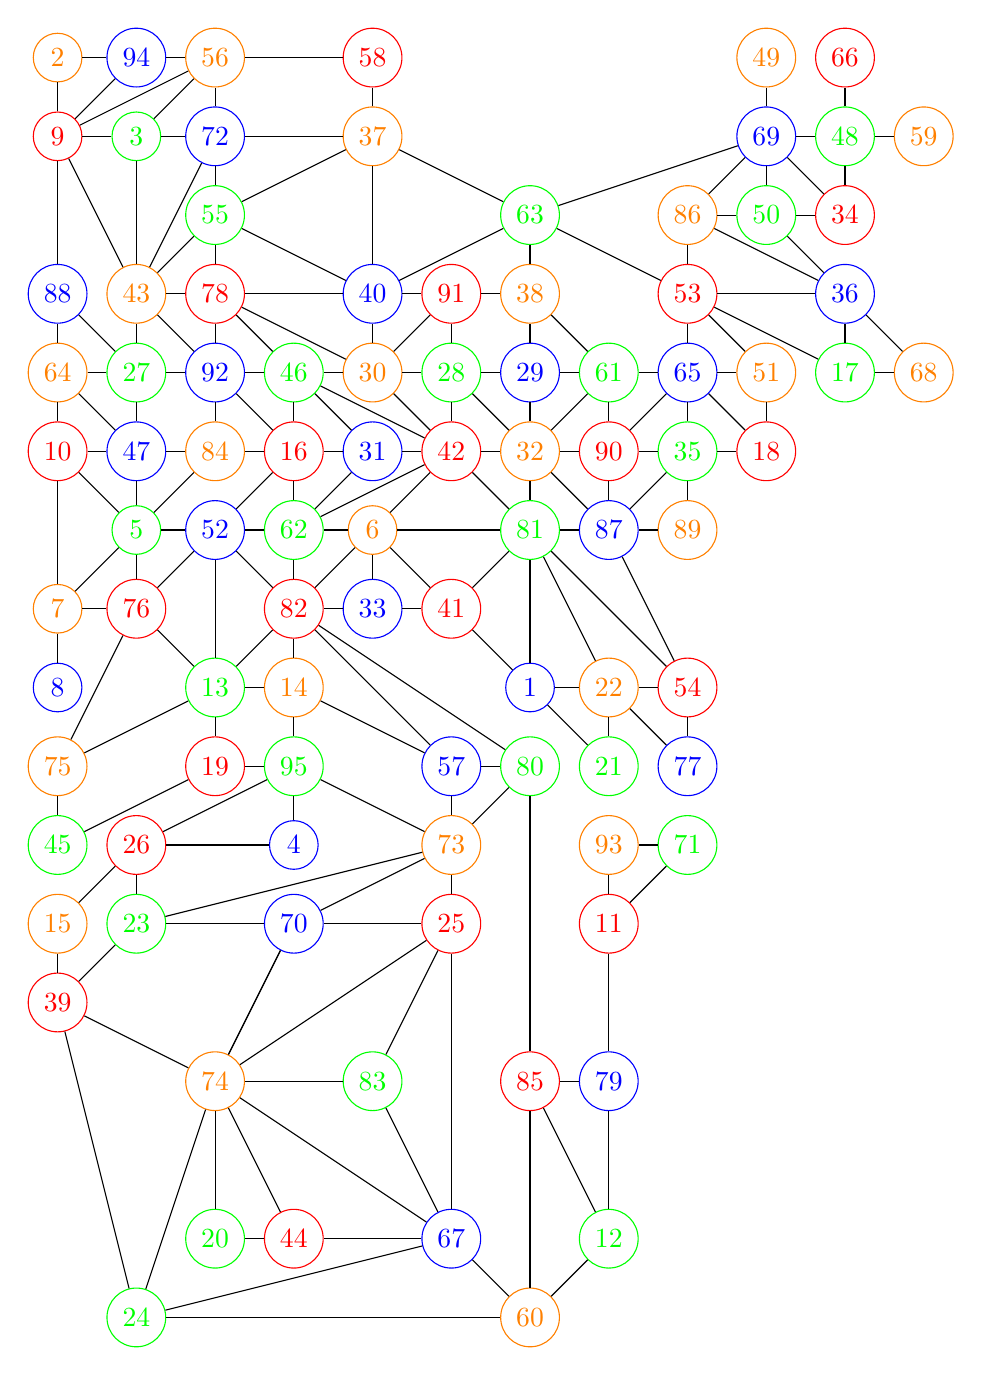
\begin{tikzpicture}
\node[circle, draw, color=blue] (AL) at (6,9){1};
\node[circle, draw, color=orange] (AK) at (0,17){2};
\node[circle, draw, color=green] (AB) at (1,16){3};
\node[circle, draw, color=blue] (Agu) at (3,7){4};
\node[circle, draw, color=green] (AZ) at (1,11){5};
\node[circle, draw, color=orange] (AR) at (4,11){6};
\node[circle, draw, color=orange] (BCN) at (0,10){7};
\node[circle, draw, color=blue] (BCS) at (0,9){8};
\node[circle, draw, color=red] (BC) at (0,16){9};
\node[circle, draw, color=red] (CA) at (0,12){10};
\node[circle, draw, color=red] (Cam) at (7,6){11};
\node[circle, draw, color=green] (Chp) at (7,2){12};
\node[circle, draw, color=green] (Chi) at (2,9){13};
\node[circle, draw, color=orange] (Coa) at (3,9){14};
\node[circle, draw, color=orange] (Col) at (0,6){15};
\node[circle, draw, color=red] (CO) at (3,12){16};
\node[circle, draw, color=green] (CT) at (10,13){17};
\node[circle, draw, color=red] (DE) at (9,12){18};
\node[circle, draw, color=red] (Dur) at (2,8){19};
\node[circle, draw, color=green] (Fed) at (2,2){20};
\node[circle, draw, color=green] (FL) at (7,8){21};
\node[circle, draw, color=orange] (GA) at (7,9){22};
\node[circle, draw, color=green] (Gto) at (1,6){23};
\node[circle, draw, color=green] (Gue) at (1,1){24};
\node[circle, draw, color=red] (Hid) at (5,6){25};
\node[circle, draw, color=red] (Jal) at (1,7){26};
\node[circle, draw, color=green] (ID) at (1,13){27};
\node[circle, draw, color=green] (IL) at (5,13){28};
\node[circle, draw, color=blue] (IN) at (6,13){29};
\node[circle, draw, color=orange] (IA) at (4,13){30};
\node[circle, draw, color=blue] (KS) at (4,12){31};
\node[circle, draw, color=orange] (KY) at (6,12){32};
\node[circle, draw, color=blue] (LA) at (4,10){33};
\node[circle, draw, color=red] (ME) at (10,15){34};
\node[circle, draw, color=green] (MD) at (8,12){35};
\node[circle, draw, color=blue] (MA) at (10,14){36};
\node[circle, draw, color=orange] (MB) at (4,16){37};
\node[circle, draw, color=orange] (MI) at (6,14){38};
\node[circle, draw, color=red] (Mch) at (0,5){39};
\node[circle, draw, color=blue] (MN) at (4,14){40};
\node[circle, draw, color=red] (MS) at (5,10){41};
\node[circle, draw, color=red] (MO) at (5,12){42};
\node[circle, draw, color=orange] (MT) at (1,14){43};
\node[circle, draw, color=red] (Mor) at (3,2){44};
\node[circle, draw, color=green] (Nay) at (0,7){45};
\node[circle, draw, color=green] (NE) at (3,13){46};
\node[circle, draw, color=blue] (NV) at (1,12){47};
\node[circle, draw, color=green] (NB) at (10,16){48};
\node[circle, draw, color=orange] (NL) at (9,17){49};
\node[circle, draw, color=green] (NH) at (9,15){50};
\node[circle, draw, color=orange] (NJ) at (9,13){51};
\node[circle, draw, color=blue] (NM) at (2,11){52};
\node[circle, draw, color=red] (NY) at (8,14){53};
\node[circle, draw, color=red] (NC) at (8,9){54};
\node[circle, draw, color=green] (ND) at (2,15){55};
\node[circle, draw, color=orange] (NW) at (2,17){56};
\node[circle, draw, color=blue] (NLe) at (5,8){57};
\node[circle, draw, color=red] (Nu) at (4,17){58};
\node[circle, draw, color=orange] (NS) at (11,16){59};
\node[circle, draw, color=orange] (Oax) at (6,1){60};
\node[circle, draw, color=green] (OH) at (7,13){61};
\node[circle, draw, color=green] (OK) at (3,11){62};
\node[circle, draw, color=green] (ON) at (6,15){63};
\node[circle, draw, color=orange] (OR) at (0,13){64};
\node[circle, draw, color=blue] (PA) at (8,13){65};
\node[circle, draw, color=red] (PEI) at (10,17){66};
\node[circle, draw, color=blue] (Pue) at (5,2){67};
\node[circle, draw, color=orange] (RI) at (11,13){68};
\node[circle, draw, color=blue] (QC) at (9,16){69};
\node[circle, draw, color=blue] (Que) at (3,6){70};
\node[circle, draw, color=green] (QR) at (8,7){71};
\node[circle, draw, color=blue] (SK) at (2,16){72};
\node[circle, draw, color=orange] (SLP) at (5,7){73};
\node[circle, draw, color=orange] (Mex) at (2,4){74};
\node[circle, draw, color=orange] (Sin) at (0,8){75};
\node[circle, draw, color=red] (Son) at (1,10){76};
\node[circle, draw, color=blue] (SC) at (8,8){77};
\node[circle, draw, color=red] (SD) at (2,14){78};
\node[circle, draw, color=blue] (Tab) at (7,4){79};
\node[circle, draw, color=green] (Tam) at (6,8){80};
\node[circle, draw, color=green] (TN) at (6,11){81};
\node[circle, draw, color=red] (TX) at (3,10){82};
\node[circle, draw, color=green] (Tla) at (4,4){83};
\node[circle, draw, color=orange] (UT) at (2,12){84};
\node[circle, draw, color=red] (Ver) at (6,4){85};
\node[circle, draw, color=orange] (VT) at (8,15){86};
\node[circle, draw, color=blue] (VA) at (7,11){87};
\node[circle, draw, color=blue] (WA) at (0,14){88};
\node[circle, draw, color=orange] (DC) at (8,11){89};
\node[circle, draw, color=red] (WV) at (7,12){90};
\node[circle, draw, color=red] (WI) at (5,14){91};
\node[circle, draw, color=blue] (WY) at (2,13){92};
\node[circle, draw, color=orange] (Yuc) at (7,7){93};
\node[circle, draw, color=blue] (YK) at (1,17){94};
\node[circle, draw, color=green] (Zac) at (3,8){95};



\foreach \from/\to in {BCS/BCN,BCN/Son,Son/Sin,Son/Chi,Sin/Chi,Sin/Nay,Nay/Dur,Chi/Dur,Chi/Coa,Col/Mch,Col/Jal,Dur/Zac,Coa/Zac,Jal/Zac,Jal/Gto,Mch/Gto,Mch/Gue,Jal/Agu,Coa/NLe,NLe/SLP,NLe/Tam,SLP/Tam,Tam/Ver,Ver/Tab,Tab/Chp,Ver/Chp,Pue/Oax,Ver/Oax,SLP/Zac,Gto/SLP,SLP/Hid,Hid/Pue,Agu/Zac,Que/SLP,Que/Gto,Que/Hid,Hid/Tla,Yuc/QR,Yuc/Cam,Cam/QR,Cam/Tab,Fed/Mex,Fed/Mor,Mex/Mch,Mex/Que,Mex/Hid,Mex/Que,Mex/Mor,Mex/Tla,Mex/Pue,Mex/Gue,Oax/Chp,Gue/Oax,Pue/Tla,Pue/Mor,Pue/Gue,YK/BC,YK/AK,BC/AK,YK/NW,BC/AB,BC/NW,BC/WA,BC/MT,AB/MT,AB/SK,AB/NW,SK/NW,SK/MB,SK/MT,SK/ND,NW/Nu,MB/Nu,MB/ON,MB/ND,MB/MN,ON/MN,ON/MI,ON/NY,ON/QC,QC/VT,QC/NH,QC/ME,QC/NB,QC/NL,NB/PEI,NB/NS,NB/ME,AL/FL,AL/GA,AL/TN,AL/MS,AZ/Son,AZ/BCN,AZ/CA,AZ/NV,AZ/NM,AZ/UT,AR/MO,AR/OK,AR/TX,AR/LA,AR/MS,AR/TN,CA/NV,CA/OR,CA/BCN,CO/UT,CO/NM,CO/KS,CO/OK,CO/WY,CO/NE,CT/MA,CT/RI,CT/NY,DE/NJ,DE/PA,DE/MD,FL/GA,GA/TN,GA/SC,GA/NC,ID/WA,ID/OR,ID/NV,ID/WY,ID/MT,ID/WY,IL/IN,IL/IA,IL/WI,IL/KY,IL/MO,IN/MI,IN/OH,IN/KY,IA/MN,IA/MO,IA/WI,IA/SD,IA/NE,KS/MO,KS/OK,KS/NE,KY/MO,KY/TN,KY/OH,KY/VA,KY/WV,LA/MS,LA/TX,ME/NH,MD/VA,MD/WV,MD/PA,MD/DE,DC/MD,DC/VA,MA/RI,MA/NH,MA/VT,MA/NY,MI/OH,MI/WI,MN/ND,MN/SD,MN/WI,MS/TN,MO/NE,MO/KS,MO/OK,MO/TN,MT/ND,MT/SD,MT/WY,NE/WY,NE/SD,NV/UT,NV/OR,NH/VT,NJ/NY,NJ/PA,NM/OK,NM/TX,NY/VT,NY/PA,NC/SC,NC/TN,NC/VA,ND/SD,OH/WV,OH/PA,OK/TX,OR/WA,PA/WV,SD/WY,TN/VA,UT/WY,VA/WV,NM/Son,NM/Chi,TX/Chi,TX/Coa,TX/NLe,TX/Tam}
 \draw (\from) -- (\to);
\end{tikzpicture}
\]

%\end{landscape}
\end{document}